\documentclass[../../main]{subfiles}

\renewcommand\thesection{\arabic{section}}


\begin{document}

\section{Buffer / Inverter} \label{sec:bufferOrInverter}

The custom boards we will be designing in the coming sections will require \emph{buffers}
here and there in order to strengthen signals, so this section introduces a simple
RTL\footnote{Resister Transistor Logic} buffer. Additionally, these \emph{boards} require
some other \emph{logic gates} too. One among them is an \emph{inverter}.

If we want to design an RTL buffer, we could simply \emph{cascade} two inverters. But we
could save one inverter, if we choose to use an \emph{inverter} as a \emph{buffer} at
the cost of \emph{flipping} the logic.

\alertNote{
    Since we are using an \emph{inverter} as a \emph{buffer}, the input logic to the
    \emph{buffer} also \emph{inverts}. If we want the output to be \emph{high} then
    the input to the buffer should be \emph{low}, so the rest of the circuit is needed to
    be designed accordingly with this change in mind.
}

We have some design requirements. These inverts / buffers are either driven by
\textbf{74LS}\footnote{They are TTL based.} ICs or \esp. \textbf{74LS} ICs are known
for their low $\si{V}_{OH}$ and low source current. Logic high of \textbf{74LS} series ranges
from $2.2\si{V}$ to $3\si{V}$. And can only source upto $0.4\si{mA}$. So we need to
design an inverter with this in mind.

We need to choose a BJT that can be driven with a small input current. \emph{BC547} is
good candidate for our scenario. Refer Figure \ref{fig:bc547Pinout} for pinout and Table
\ref{tbl:bc547Spec} for a brief specification of \emph{BC547}.

\begin{center}
    {\begin{minipage}[c] {0.42\textwidth}
        \centering
        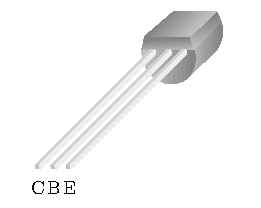
\includegraphics [
        ] {pics/bc547.pdf}
        \captionof{figure} {
            Pinout of \textbf{BC547}.
            \label{fig:bc547Pinout}
        }
    \end{minipage}
    \begin{minipage}[c] {0.52\textwidth}

        \begin{tabularx} {\linewidth} {
                *{1}{>{\centering\arraybackslash}m{0.3\linewidth}}
                *{1}{>{\centering\arraybackslash}m{0.7\linewidth}}
            }
            \toprule
            Parameter & Value \\
            \midrule
            $\si{V}_{CEO}$ Max. & $45 \si{V}$ \\
            $\si{V}_{EBO}$ Max. & $6 \si{V}$ \\
            $\si{I}_{C}$ Max. & $100 \si{mA}$ \\
            $\si{P}_{C}$ Max. & $500 \si{mW}$ \\
            $\si{C}_{ob}$ (Output Capacitance) Max. & $6 \si{pF}$ \\
            \bottomrule
        \end{tabularx}
        \captionof{table} {
            Brief specification of \textbf{BC547}.
            \label{tbl:bc547Spec}
        }
    \end{minipage}}

\end{center}

\begin{center}
    {\begin{minipage} [c] {0.55\textwidth}
        Figure \ref{fig:clvlInverter} shows an RTL inverter implemented using \emph{BC547}.
        Now we need to choose the resisters $\si{R}_{b}$ and $\si{R}_{c}$. $\si{R}_{b}$
        is needed to be selected such that it will sink only the necessary amount of current
        that is needed to drive \emph{BC547}. \resValOneFiveK{} seems like a best bet, because if we
        choose \resValOneFiveK{}, the $\si{I}_{b}$ with $\si{V}_{in} = 3\si{V}$ would
        be:

        \begin{align}
            \si{I}_{b} &= \dfrac{3 \si{V}}{15\si{k \ohm}} \\
            &= 0.2 \si{mA}
        \end{align}

        Which is just below the maximum source current \textbf{74LS} series can provide.

    \end{minipage}
    \hfill
    \begin{minipage} [c] {0.35\textwidth}
        \centering
        \includegraphics [
            max width = \IGXMaxWidth,
            max height = \IGXMaxHeight,
            \IGXDefaultOptionalArgs,
        ] {tikzpics/endClvlInverter.pdf}
        \captionof{figure} {A simple RTL inverter using \emph{BC547}.}
        \label{fig:clvlInverter}
    \end{minipage}\hfill}
\end{center}

\alertWarning{
    It is not necessary to use a \emph{low} $\si{R}_{b}$ in this case\footnote{here with a
    \resValOneFiveK{} resister.}. Because \emph{BC547} can be driven with $\si{\mu A}$ range base current.
    As we will see in further chapters, \emph{74LS} IC pins won't be able to drive more than $2$
    such inverters. So it is recommended to use a higher $\si{R}_{b}$ as it would only sink much
    less current from IC pins.
}

Now that out of the way, we can go ahead and choose $\si{R}_{c}$. $\si{R}_{c}$ will determine the
switching speed of the inverter. We are not planning to drive these inverters in high
frequencies\footnote{ie, maximum frequencies \emph{74LS} series is capable of (which is
around $25\si{Mhz}$ to $35\si{Mhz}$).}. We will be driving these inverters at a frequency
of $500\si{kHz}$.

From the table \ref{tbl:bc547Spec}, we can see that the maximum output capacitance of \emph{BC547}
is $6 \si{pF}$. So if we choose $\si{R}_{c}$ as \resValThreeThreeK{}, we would get the low to
high transition time as:

\begin{align}
    T_{LH} &= 33\si{k \ohm} \times 6 \si{pF} \\
    &= 1.98 \times 10^{-7} \si{s} \\
    &\approx 0.2 \si{\mu s}
\end{align}

So choosing $\si{R}_{c}$ as \resValThreeThreeK{} would result in no limitation if we want to drive
these at $500\si{kHz}$.

\alertTip{
    Just use \emph{CD 4050 BE - Hex Buffer/Converter} and \emph{74LS04 - Hex Inverter}.
}

\end{document}
